%\section{Section}
%\subsection{Subsection}
\begin{frame}{Chronology}
	\begin{table}
		\renewcommand\arraystretch{1.4}
		\begin{tabular}{@{\,}r <{\hskip 2pt} !{\timelinebullet} >{\raggedright\arraybackslash}p{0.6\textwidth}}
		2013 & [BCH] “A Model of Type Theory in Cubical Sets”\\
		2015 & [CCHM] De Morgan Cubical Type Theory\\
		2018 & [CHM] Higher Inductive Types in CuTT\\
		2019 & [VMA] Cubical Agda\\
		\end{tabular}
	\end{table}
\end{frame}

\begin{frame}<1-5>[t]{Sets as Types}
	\centering
	\bgroup
	{
		\def\arraystretch{1.5}
		\begin{tabularx}{\textwidth}{@{}>{\centering\arraybackslash}X|>{\centering\arraybackslash}X@{}}
			\textbf{Types} & \textbf{Sets}\\\hline
			$x : A$ & $x \in A$
			\only<2->{\\\hline
			\textcolor<3-4>{gray}{$\mathbf{0}$} & \textcolor<3-4>{gray}{$\emptyset$} \\
			\textcolor<3-4>{gray}{$\mathbf{1}$} & \textcolor<3-4>{gray}{$\{0\}$} \\
			\textcolor<4>{gray}{\alt<3>{$\mathsf{inl}\, x : A + B$}{$A + B$}} & \textcolor<4>{gray}{\alt<3>{$(0, x) \in A \uplus B$}{$A \uplus B$}} \\
			\textcolor<3>{gray}{\alt<4>{$(x, y) : A \times B$}{$A \times B$}} & \textcolor<3>{gray}{\alt<4>{$(x, y) \in A \times B$}{$A \times B$}} \\
			\textcolor<3-4>{gray}{$A \to B$} & \textcolor<3-4>{gray}{$B^A$} \\
			}
		\end{tabularx}
	}
	\egroup
\end{frame}

\begin{frame}<1-6>[t]{Propositions as Types}
	\centering
	\bgroup
	{
		\def\arraystretch{1.5}
		\begin{tabularx}{\textwidth}{@{}>{\centering\arraybackslash}X|>{\centering\arraybackslash}X@{}}
			\textbf{Types} & \textbf{Propositions}\\\hline
			$x : A$ & $A \mathrel{\mathsf{true}}$
			\only<2->{\\\hline
			\textcolor<3-4>{gray}{$\mathbf{0}$} & \textcolor<3-4>{gray}{$\bot$} \\
			\textcolor<3-4>{gray}{$\mathbf{1}$} & \textcolor<3-4>{gray}{$\top$} \\
			\textcolor<3-4>{gray}{$A + B$} & \textcolor<3-4>{gray}{$A \lor B$} \\
			\textcolor<4>{gray}{\alt<3>{$(x, y) : A \times B$}{$A \times B$}} & \textcolor<4>{gray}{\alt<3>{$A \land B \mathrel{\mathsf{true}}$}{$A \land B$}} \\
			\textcolor<3>{gray}{\alt<4>{$\lambda x.\,y : A \to B$}{$A \to B$}} & \textcolor<3>{gray}{\alt<4>{$A \implies B \mathrel{\mathsf{true}}$}{$A \implies B$}} \\
			}
		\end{tabularx}
	}
	\egroup

	\only<6>{This translation is known as the \textbf{Curry-Howard correspondence}.}
\end{frame}

\begin{frame}{Propositions as Types | Agda}
	\centering
	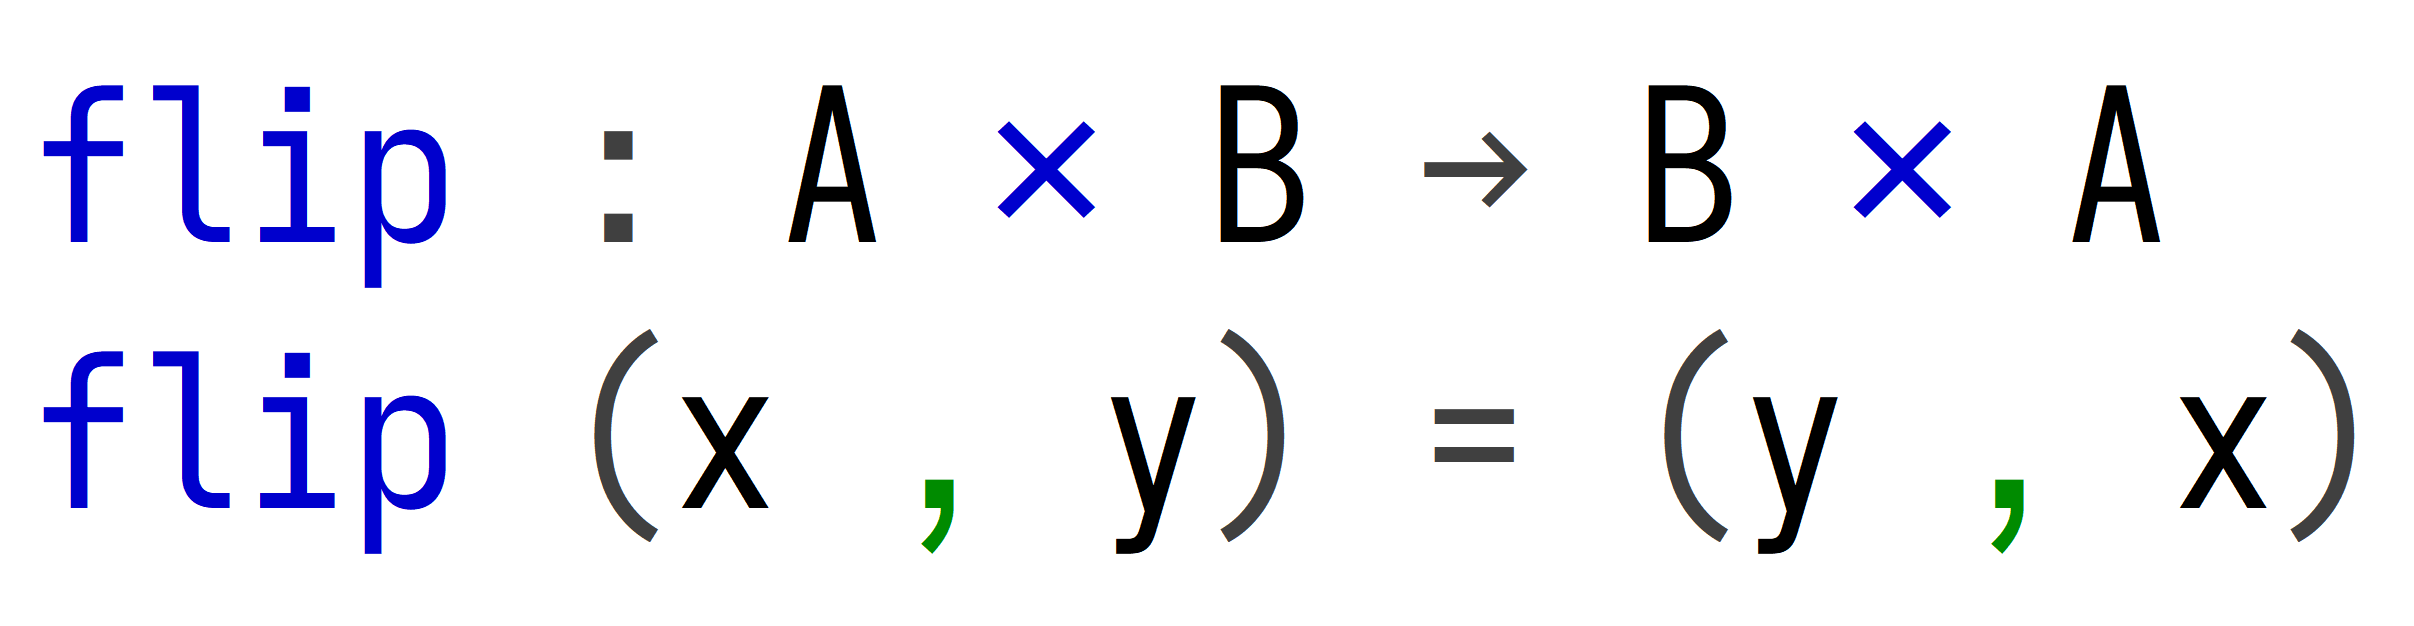
\includegraphics[height=32pt]{../res/flip-simple.png}
\end{frame}

\begin{frame}{Universes and Quantifiers}
	We're still missing some crucial type formers:
	\begin{itemize}
		\uncover<2->{\item We don't have a way to talk about types \textbf{internally}.}
		\uncover<3->{\item We don't have existential/universal \textbf{quantifiers}.}
	\end{itemize}
\end{frame}

\begin{frame}<1-3>{Universes}
	\centering
	\alt<1-2>{
		We'll add a \textbf{universe}\dots
		\begin{equation*}
			\mathcal{U}
		\end{equation*}
	}{
		We'll add a \emph{hierarchy} of \textbf{universes}\dots
		\begin{equation*}
			\mathcal{U}_0 : \mathcal{U}_1 : \mathcal{U}_2 : \cdots
		\end{equation*}
	}
	\uncover<2->{\dots closed under our type formers.}
\end{frame}

\begin{frame}<1-6>[t]{Quantifiers}
	\centering
	A \textbf{type family} $P : A \to \mathcal{U}$ represents a \textbf{predicate}.
	\vspace*{\baselineskip}

	\uncover<2->{
	\alt<2-5>{
	\bgroup
	\def\arraystretch{1.5}
	\begin{tabularx}{\textwidth}{@{}>{\centering\arraybackslash}X|>{\centering\arraybackslash}X@{}}
		\textbf{Types} & \textbf{Propositions}\\\hline
		\only<3->{$\displaystyle(x, y) : \sum_{x : A}\,P\, x$} & $\displaystyle\vphantom{\sum_{x : A}}\exists x.(x \in A) \land P(x)$
		\only<4->{\\
			\only<5->{$\displaystyle\lambda x.\, y : \prod_{x : A}\,P\, x$} & $\displaystyle\vphantom{\prod_{x : A}}\forall x.(x \in A) \implies P(x)$
		\\}
	\end{tabularx}
	\egroup
	}{
	\bgroup
	\def\arraystretch{1.5}
	\begin{tabularx}{\textwidth}{@{}>{\centering\arraybackslash}X|>{\centering\arraybackslash}X|>{\centering\arraybackslash}X@{}}
		\textbf{Sets} & \textbf{Types} & \textbf{Propositions}\\\hline
		$\displaystyle\biguplus_{x \in A}\, P(x)$ & $\displaystyle\sum_{x : A}\,P\, x$ & $\displaystyle\exists x.(x \in A) \land P(x)$\\
		$\displaystyle\prod_{x \in A}\, P(x)$ & $\displaystyle\prod_{x : A}\,P\, x$ & $\displaystyle\forall x.(x \in A) \implies P(x)$\\
	\end{tabularx}
	\egroup
	}
	}
\end{frame}


\begin{frame}{Dependent Types | Agda}
	\centering
	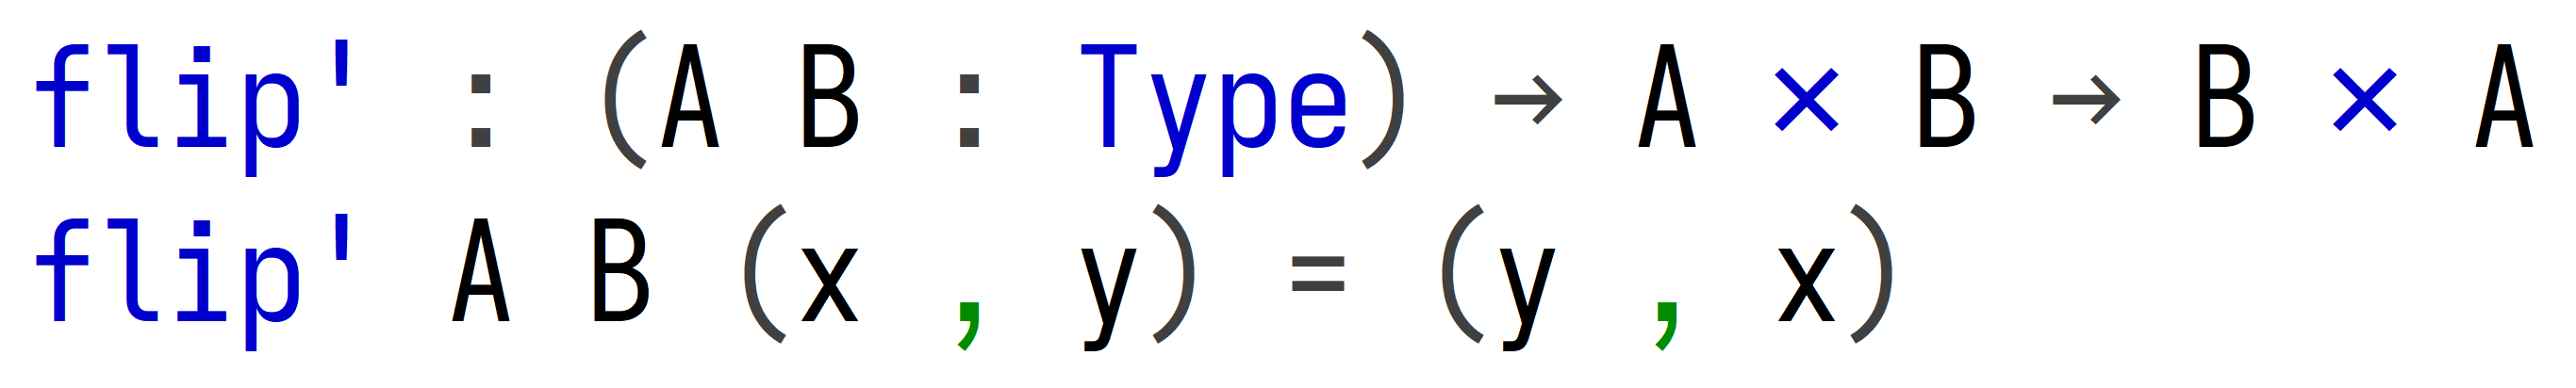
\includegraphics[height=32pt]{../res/flip-dependent.png}
\end{frame}

\begin{frame}<1-2>[label=wbequality]{What About Equality?}
	\centering
	\cleanalign{\centering}{
		\begin{gathered}
			\overbrace{\mathbf{0}\qquad\mathbf{1}\qquad\mathbf{2}\qquad\mathbb{N}\qquad{+}\qquad{\Sigma}\qquad{\times}}^\text{inductive types}\qquad{\Pi}\qquad\mathcal{U}
		\end{gathered}
	}
	
	\vspace*{\baselineskip}
	\interrule

	\uncover<2->{We'd like a type $x = y$ whose terms \textbf{witness} the fact that $x$ equals $y$.}

	\uncover<3->{Cubical type theories take inspiration from \textbf{topology}.}
\end{frame}

\begin{frame}{The Martin-L"of Identity Type}
	\centering
	We could encode equality as an \textbf{indexed inductive} \emph{identity} type.

	\bigskip
	\uncover<2->{
	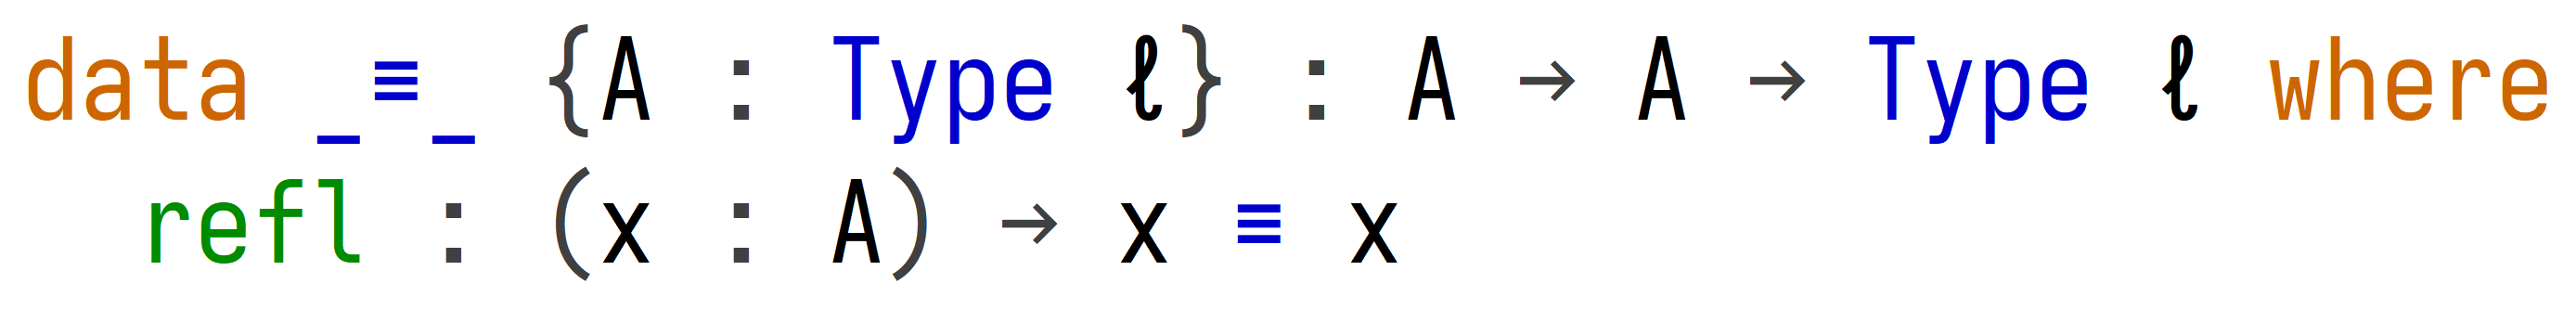
\includegraphics[height=32pt]{../res/mltt-id.png}
	}

	\uncover<3->{
	This is elegant in some ways (\emph{judgemental} path induction)\dots
	}

	\uncover<4->{
	\dots but inadequate in others (lacks \textbf{function extensionality}).
	}
\end{frame}

\againframe<3->{wbequality}

\begin{frame}{Paths, Topologically}
	\medskip
	
	\begin{columns}[b,onlytextwidth]
		\begin{column}{0.6666\textwidth}
			\centering
			\uncover<2->{
				A \textbf{path} $p$ in a topological space $X$ is a continuous map
				\begin{equation*}
				p : \mathbb{I} \to X
				\end{equation*}
				where $\mathbb{I}$ is the \textbf{unit interval} $[0, 1]$.
			}
		\end{column}
		\begin{column}{0.3333\textwidth}
			\centering
			\uncover<2->{
				\begin{tikzpicture}[scale=1,black,y=-1cm,every node/.style={scale=0.6}]
					% Points
					\coordinate (Z) at (0.5000, -0.4);
					\coordinate (U) at (1.5000, -0.4);
					\coordinate (A) at (0.5000, 0.5000);
					\coordinate (B) at (1.5000, 1.2000);

					% Space
					\draw[black,line width=1pt,fill=color_fill_default] plot [smooth cycle] coordinates {
					(1.8756, 0.6404)
					(1.1386, 0.0481)
					(0.2441, 0.2829)
					(0.0758, 1.2369)
					(0.8278, 1.9409)
					(1.7991, 1.6066)
					};
					\draw (0, 1) node[left=1pt] {$X$};
					
					% Interval
					\uncover<3->{
					\draw (Z) -- (U);

					\draw (Z) node[left=1pt] {$\mathbb{I}$};
					\draw ($(Z)+(0,0.05)$) -- ($(Z)+(0,-0.05)$) node[above] {$0$};
					\draw ($(U)+(0,0.05)$) -- ($(U)+(0,-0.05)$) node[above] {$1$};
					}

					% Path
					\only<2->{
						\draw[black, line width=1pt]
							(A)
								.. controls (1.046, 0.616) and (0.984, 1.142) ..
							(B);
						\draw (1, 1) node[below left] {$p$};
					}

					% Endpoints
					\only<4->{
						\draw[dashed] (Z) -- (A);
						\draw[dashed] (U) -- (B);
						\fill[black] (A) circle(1.4pt) node[below=1pt] {$p_0$};
						\fill[black] (B) circle(1.4pt) node[below=1pt] {$p_1$};
					}
				\end{tikzpicture}
			}
		\end{column}
	\end{columns}

	\interrule

	\uncover<5->{
		\centering
		What if we treat a type as a kind of space,

		where two points are \textit{equal} iff they are connected by a path?
		\par
	}
\end{frame}